\documentclass [12pt] {article}
\makeatletter
\setlength{\@fptop}{0pt}
\makeatother
\usepackage{graphicx}
\usepackage{color}
\usepackage{listings}
\lstset{ %
language=C++,                % choose the language of the code
basicstyle=\footnotesize,       % the size of the fonts that are used for the code
numbers=left,                   % where to put the line-numbers
numberstyle=\footnotesize,      % the size of the fonts that are used for the line-numbers
stepnumber=1,                   % the step between two line-numbers. If it is 1 each line will be numbered
numbersep=5pt,                  % how far the line-numbers are from the code
backgroundcolor=\color{white},  % choose the background color. You must add \usepackage{color}
showspaces=false,               % show spaces adding particular underscores
showstringspaces=false,         % underline spaces within strings
showtabs=false,                 % show tabs within strings adding particular underscores
frame=single,           % adds a frame around the code
tabsize=2,          % sets default tabsize to 2 spaces
captionpos=b,           % sets the caption-position to bottom
breaklines=true,        % sets automatic line breaking
breakatwhitespace=false,    % sets if automatic breaks should only happen at whitespace
escapeinside={\%*}{*)}          % if you want to add a comment within your code
}

\title{\vspace{-2cm}Assignment \#5: Silver Springs Model}
\author{Timmy Nguyen}
\begin{document}
\maketitle
\section{A Brief Introduction}
In this assignment, we learn how energy flows in a system using the Silver Springs model. Here the trophic levels are represented P, H, C1, C2 and D -- producers, herbivores, carnivores, top carnivores, and decomposers. Below are the figures representing the model and the results generated.
\section{Results}

\subsubsection{Silver Springs Aquatic Model}
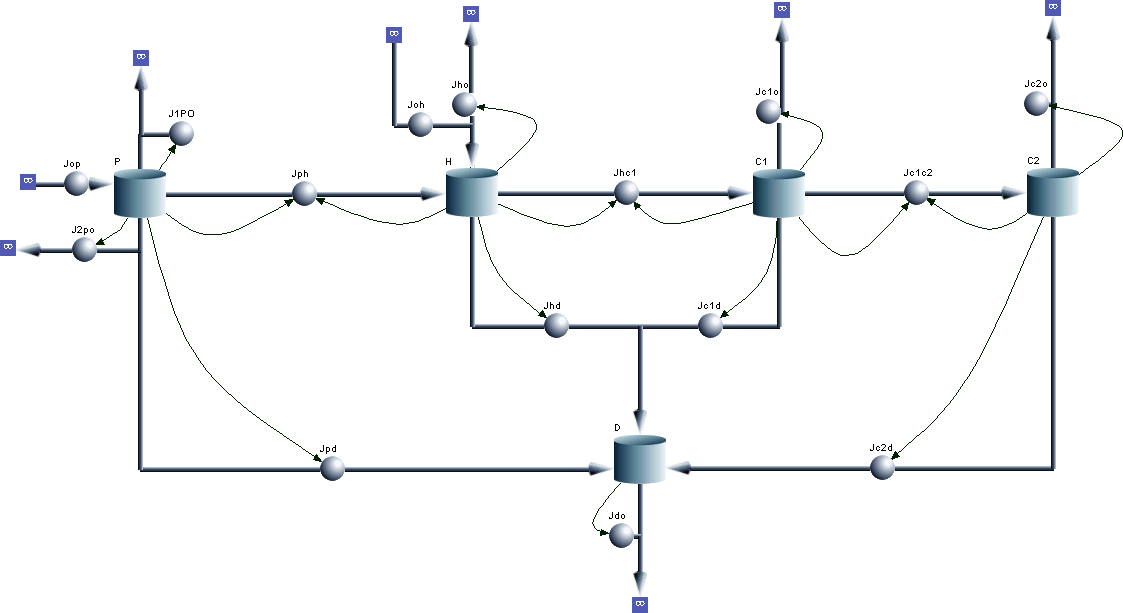
\includegraphics[scale=0.4]{silver_spring_model.png} \\
% 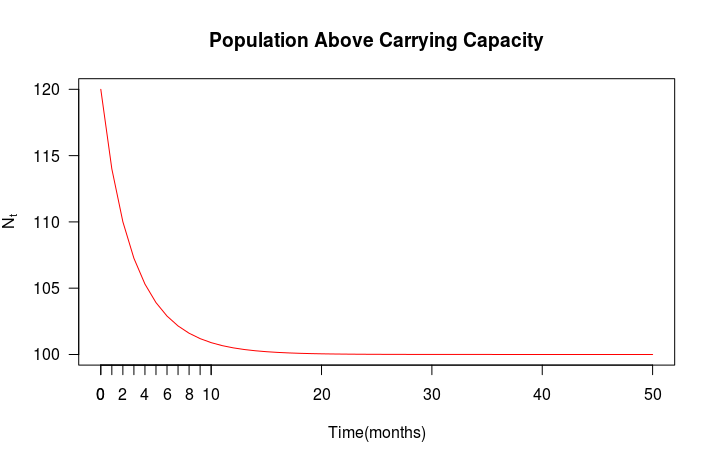
\includegraphics[scale=0.6]{graph2.png}
\newpage


\subsubsection{P and H over Time}
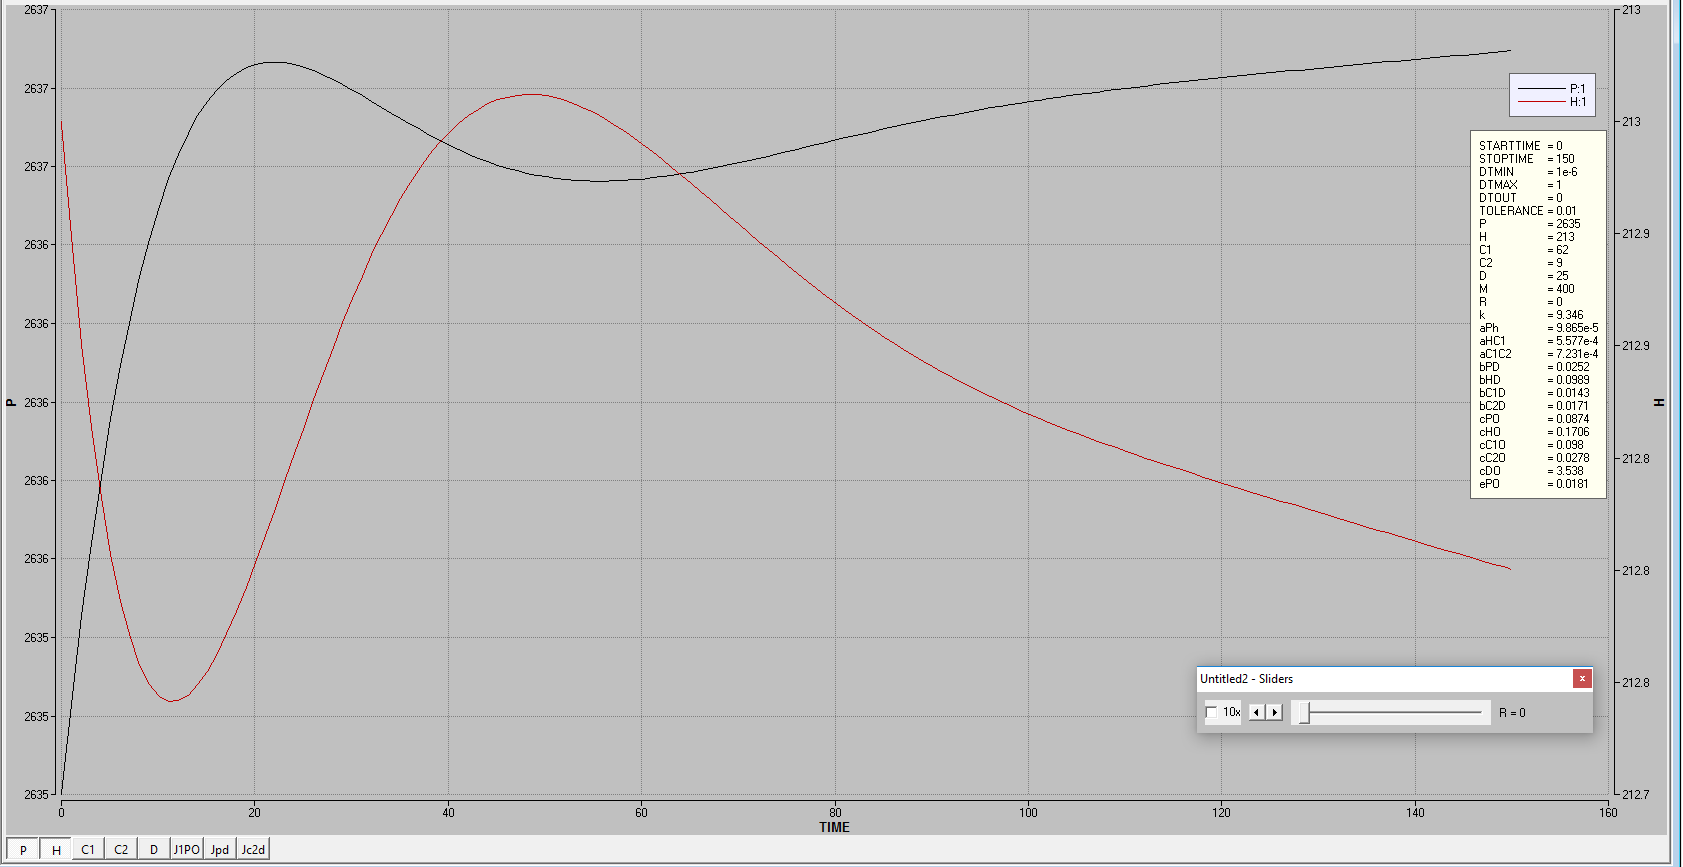
\includegraphics[scale=0.3]{graph1a.png} \\
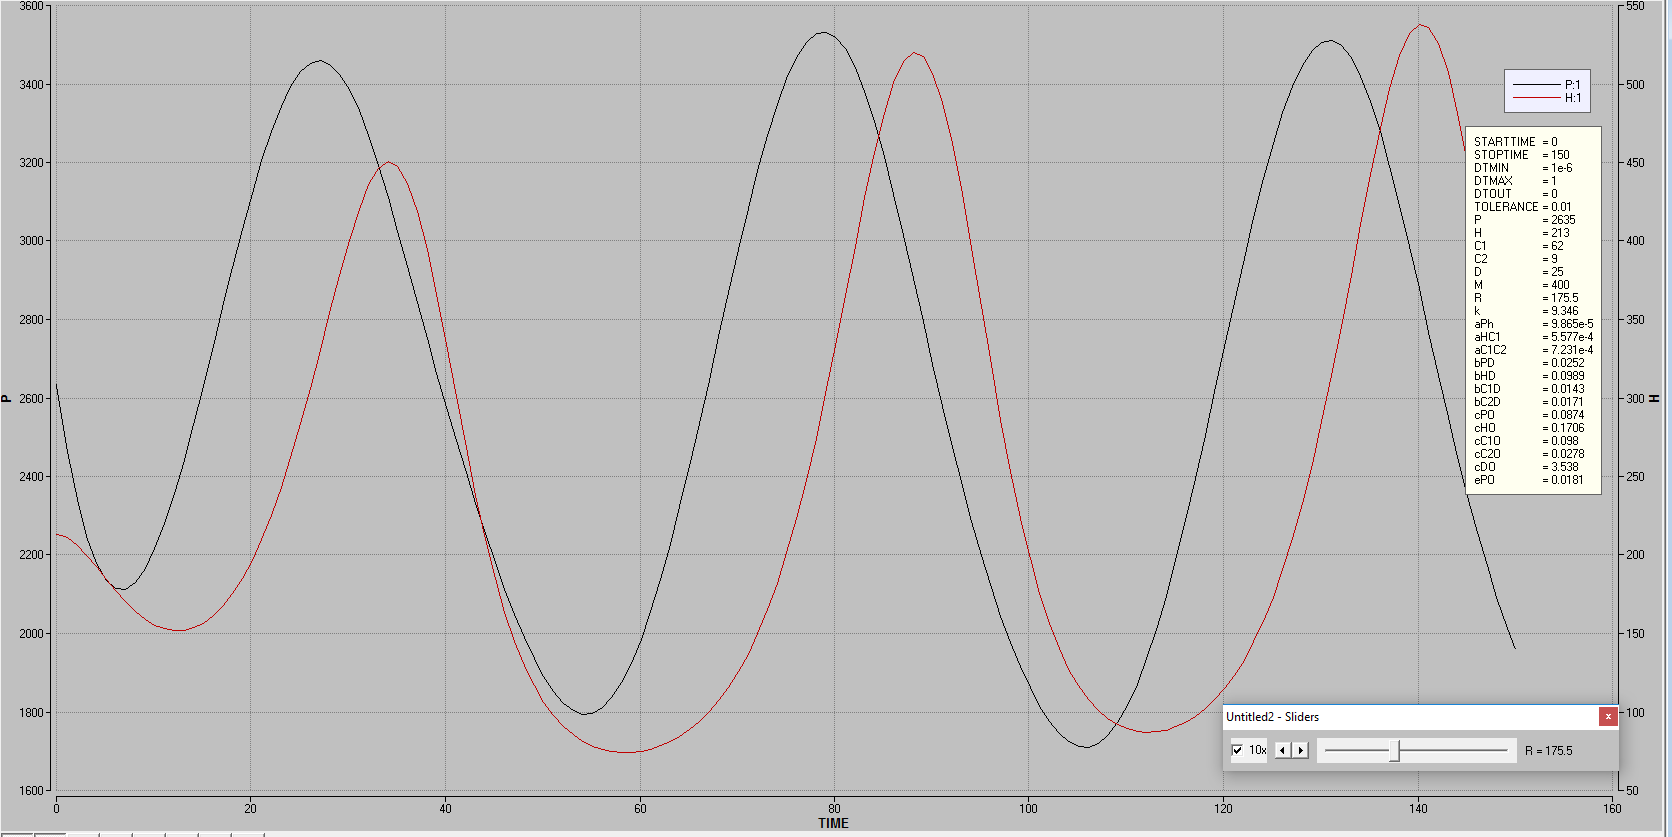
\includegraphics[scale=0.3]{graph1b.png}





\subsection{H and C1 over Time}
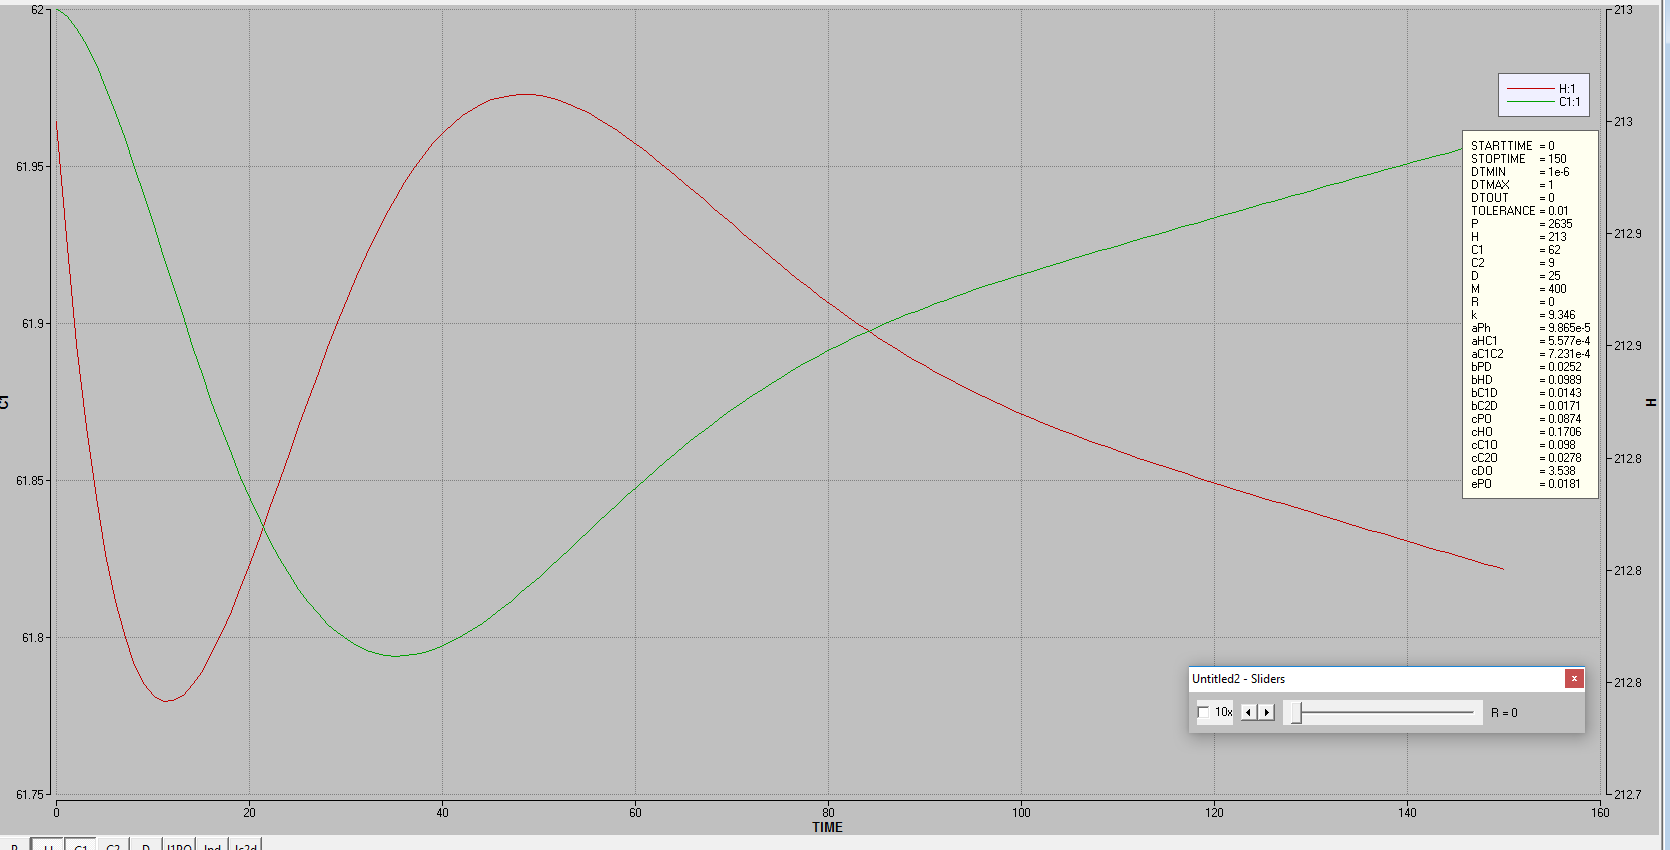
\includegraphics[scale=0.3]{graph2a.png} \\
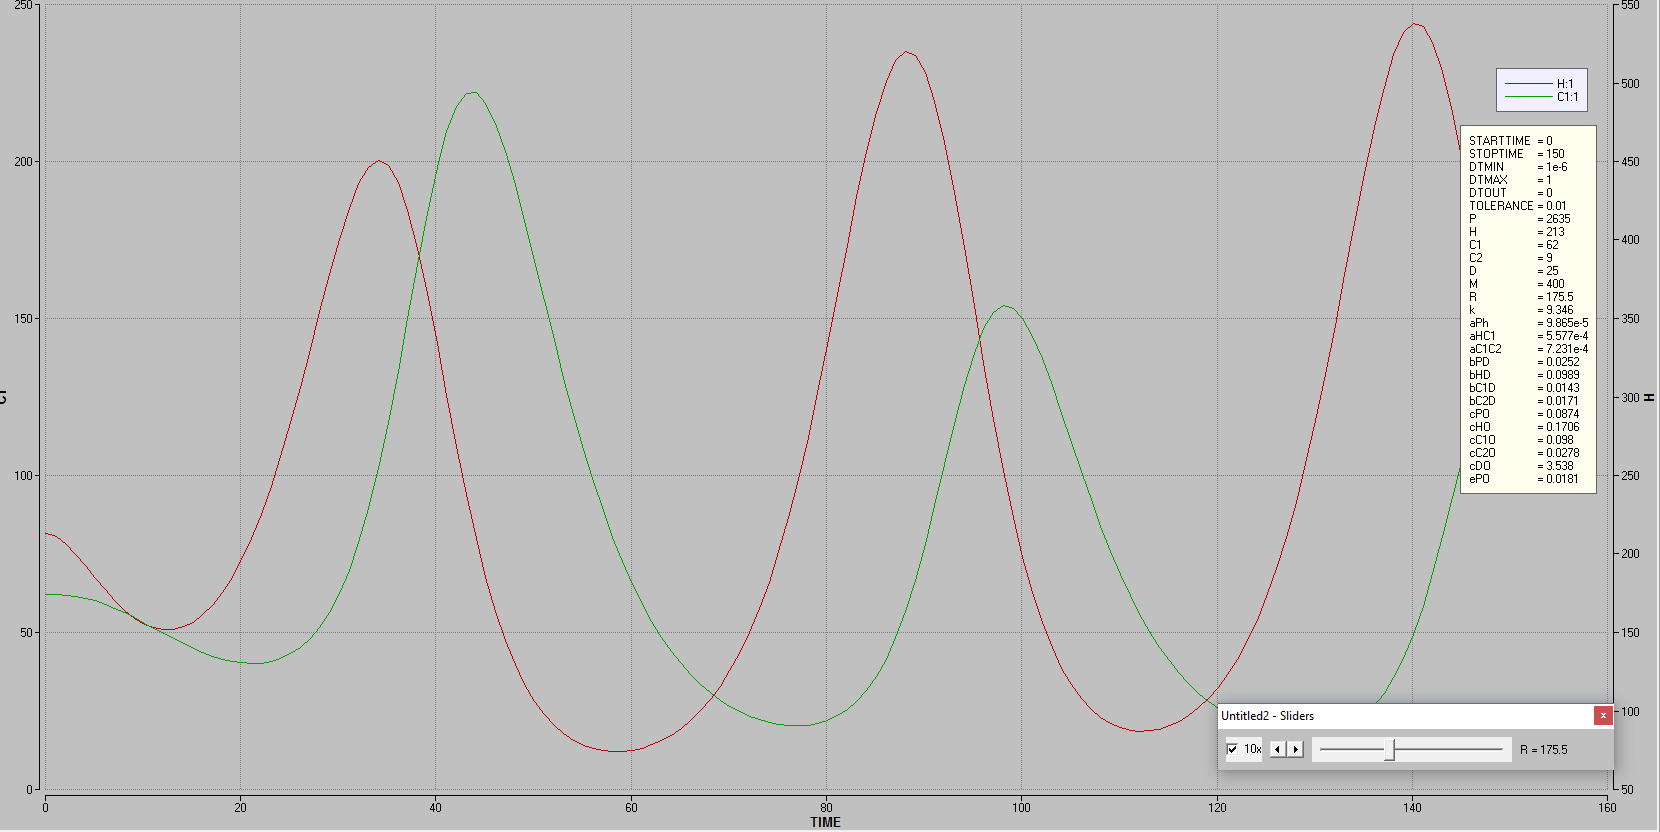
\includegraphics[scale=0.3]{graph2b.png}

\subsection{H and C2 over Time}
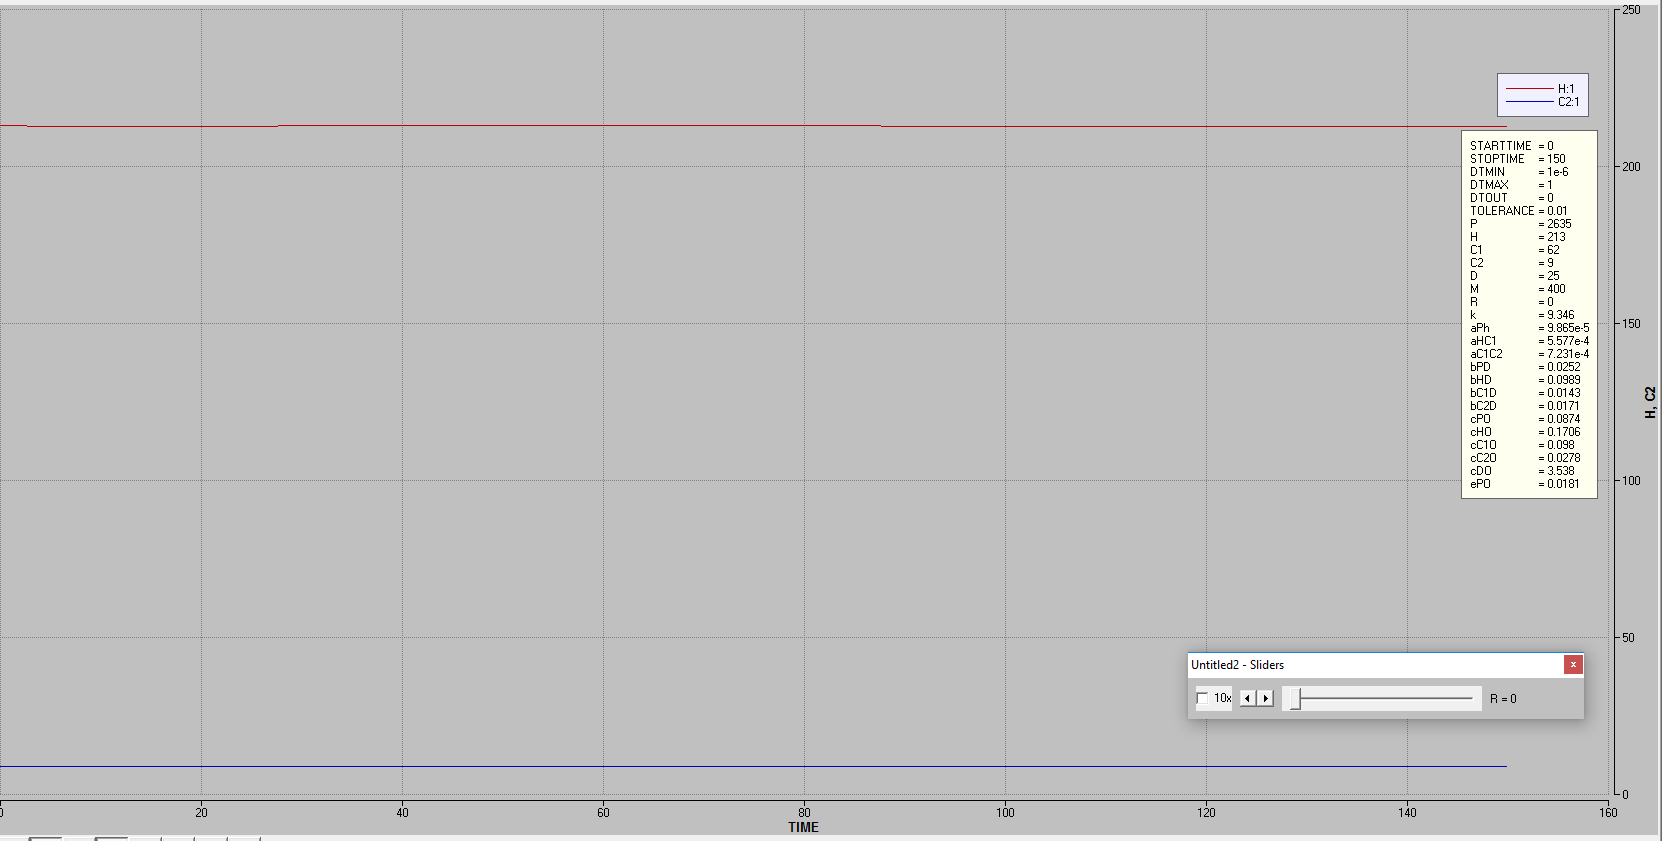
\includegraphics[scale=0.3]{graph3a.png} \\
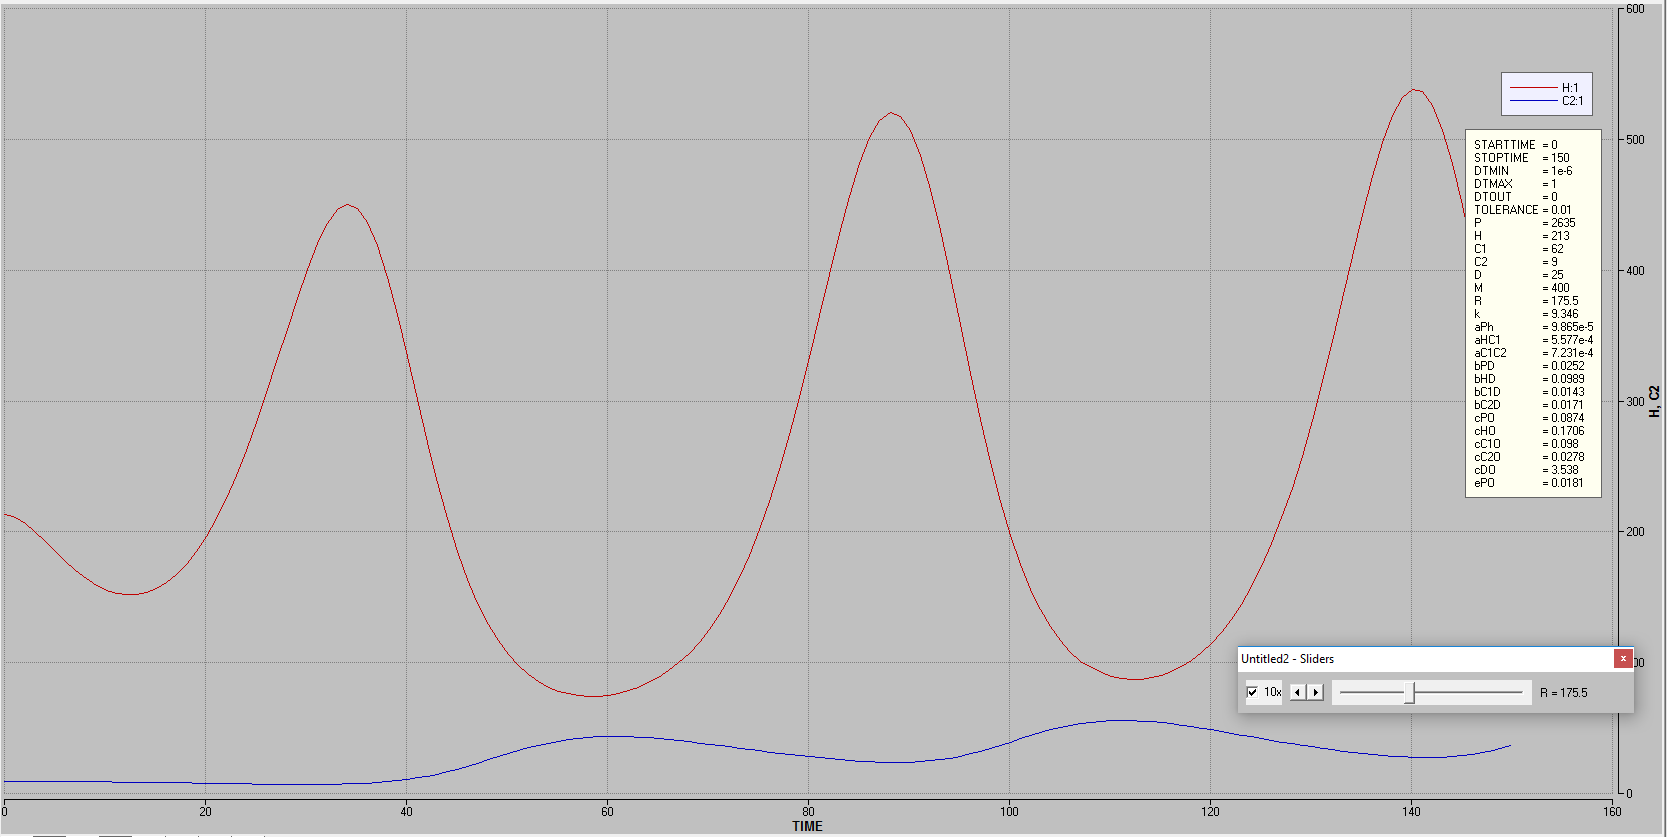
\includegraphics[scale=0.3]{graph3b.png}

\subsection{H and D over Time}
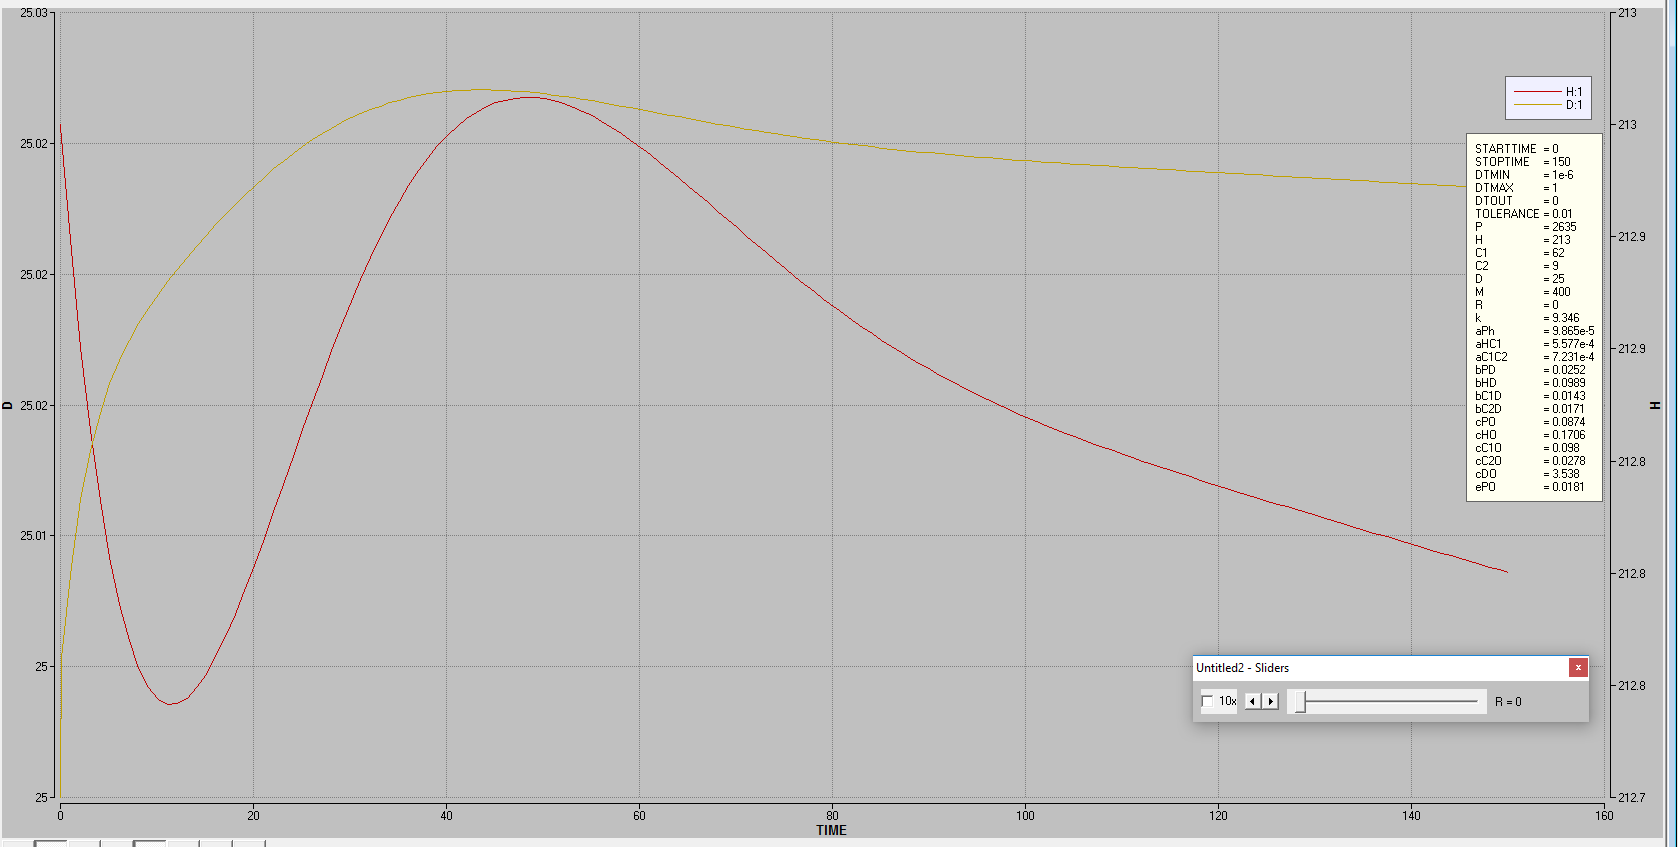
\includegraphics[scale=0.3]{graph4a.png} \\
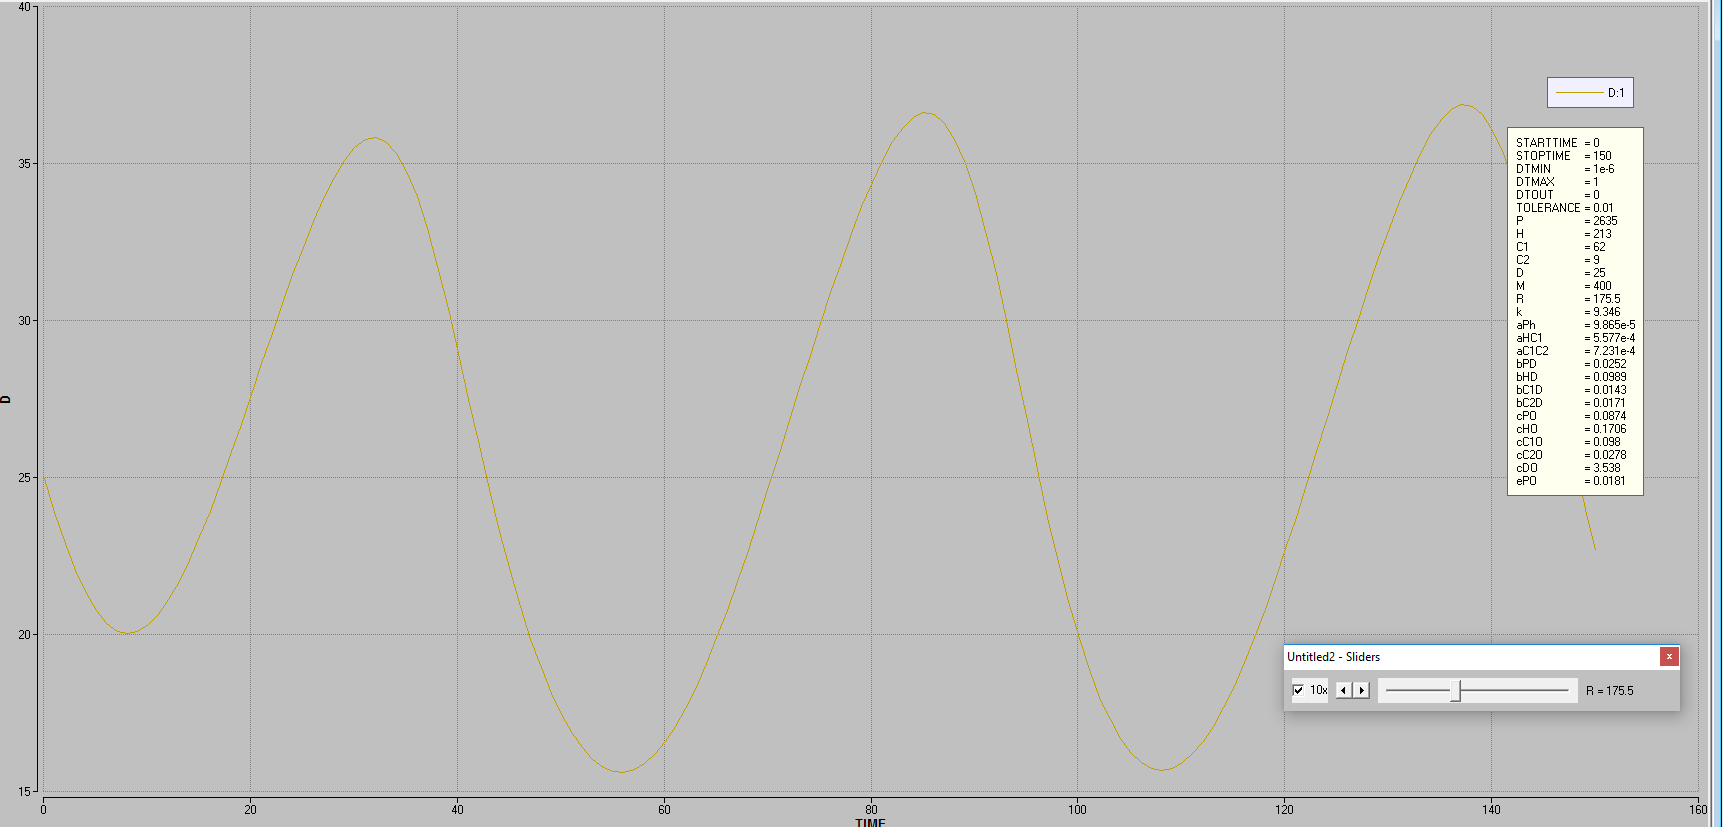
\includegraphics[scale=0.3]{graph4b.png}

\section{Conclusion}
The driving forces in this model are \textit{Jop} and \textit{Joh}. They represent the energy input from the sun and the energy input from bread feeding. As energy flows into each trophic level, much of the energy is either lost as heat or waste which would then be consume by the decomposers.  In the graph of \textit{P and H}, energy output from producers takes time to build up due to photosynthesis where herbivores has to to wait for the producers to build up energy. In the graph of \textit{H and C1}, carnivores outputs less energy. Lastly, Decomposer energy increases as Herbivores increases.
\newpage

\section{Appendix}
% \subsubsection{C/C++ Code for Exponential Growth Model}
% \lstinputlisting[language=c]{Predator_Prey_model.cpp}
% \subsubsection{R Code for Generating Predator and Prey Population Size Over Time}
% \lstinputlisting[language=R]{Predator_Prey_Model.R}

% \subsectio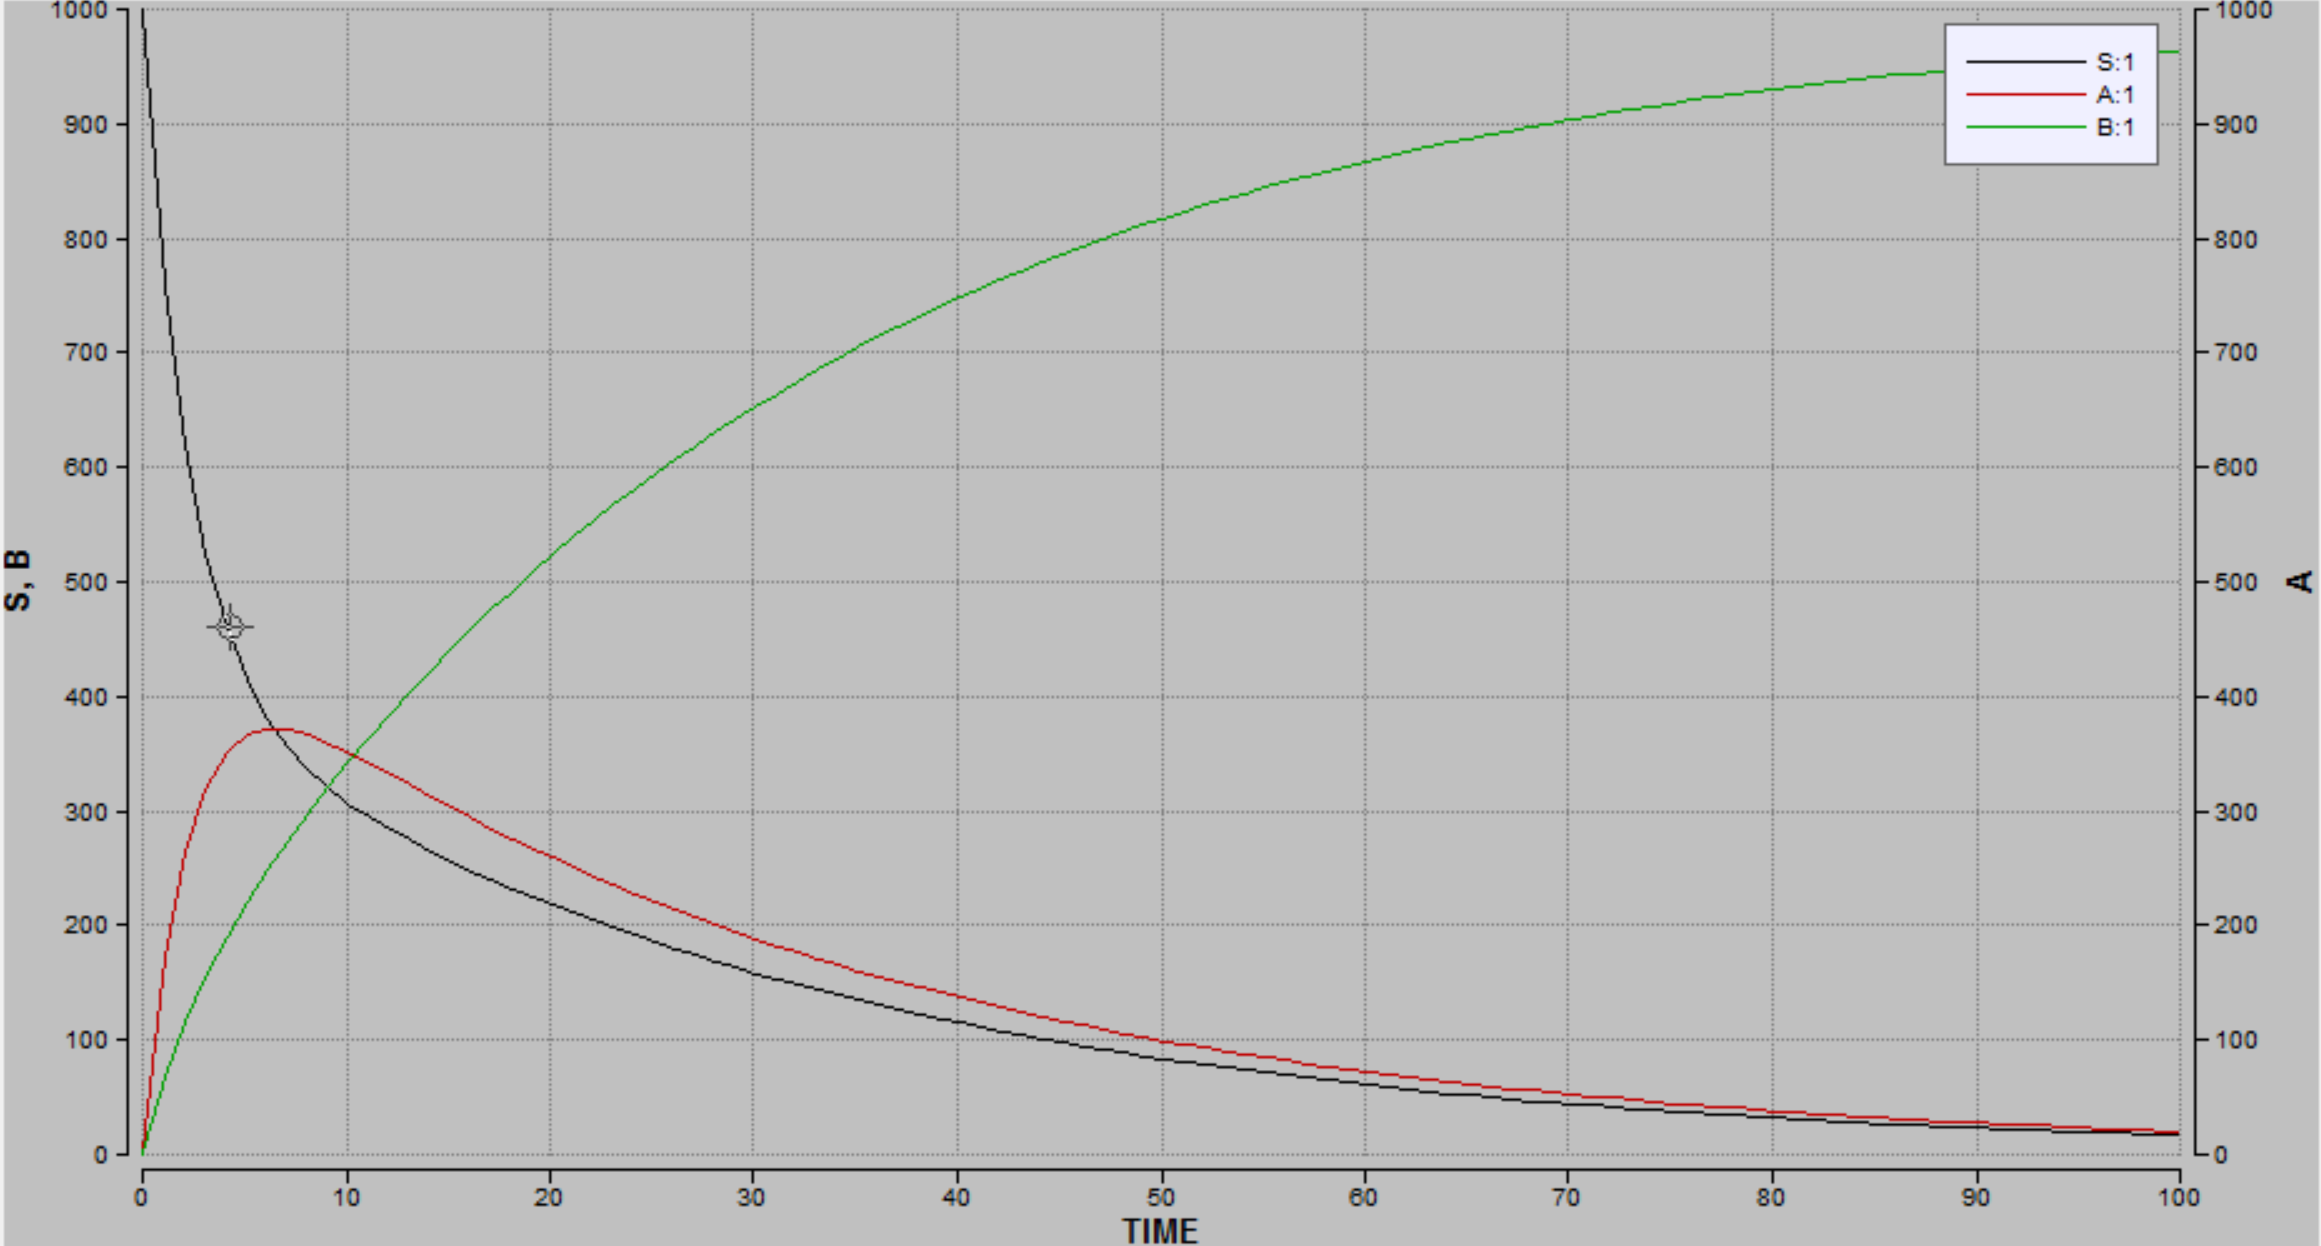
\includegraphics[scale=0.7]{ksb_less_ksa.PNG}n{R code for Generating Predator vs Prey Population Size }
% \lstinputlisting[language=R]{Predator_VS_Prey_Graph.R}
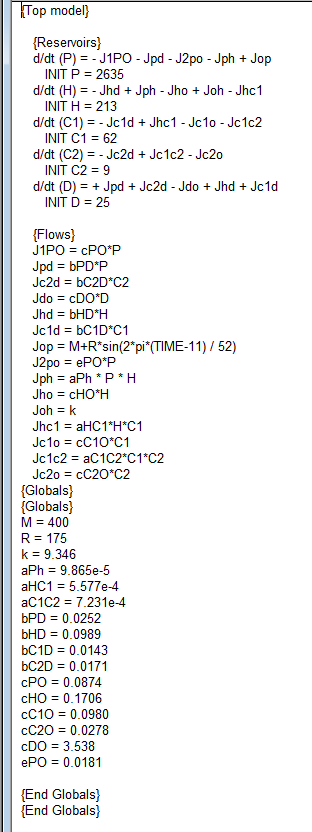
\includegraphics[scale=0.7]{silver_spring_equation.png}

\end{document}

